\documentclass{article}
\usepackage[utf8]{inputenc}
\usepackage{amsmath}
\usepackage{amssymb}
\usepackage{graphicx}

\begin{document}

\section*{Linear Data Fitting}
We are given a function $f$ and certain measured points $\left(t_{i}, f\left(t_{i}\right)\right)$. The function $f\left(t\right)$ is assumed to be a linear combination
\begin{equation*}
    f\left(t\right) = \sum_{j=1}^{4}\gamma_{i}\phi_{j}\left(t\right)
\end{equation*}
of the functions
\begin{equation*}
    \phi_{1}\left(t\right) = \frac{1}{t}, \quad \phi_{2}\left(t\right) = \frac{1}{t^{2}}, \quad \phi_{3}\left(t\right) = e^{-\left(t-1\right)}, \quad \phi_{4}\left(t\right) = e^{-2\left(t-1\right)}
\end{equation*}
We aim to calculating the coefficients $\gamma_{i}, j = 1,2,3,4$ such that
\begin{equation*}
\sum_{i=1}^{10}\left(f\left(t_{i}\right) - f_{i}\right)^{2} \longrightarrow \text{min}
\end{equation*}
\subsection*{3-3.a}
We are tasked with computing a least squares estimate for the coefficients $\gamma_{i}$ given the above information. We are told to use the normal equations to solve the problem. Given the input \verb|t| containing values and \verb|f| containing the values of $f$ evaluated at these points, we get equations of the following form.
\begin{align*}
    &\gamma_{1}\frac{1}{t_{1}} + \gamma_{2}\frac{1}{t_{1}^{2}} + \gamma_{3}e^{-\left(t_{1}-1\right)} + \gamma_{4}e^{-2\left(t_{1}-1\right)} = f\left(t_{1}\right)\\
    &\gamma_{1}\frac{1}{t_{2}} + \gamma_{2}\frac{1}{t_{2}^{2}} + \gamma_{3}e^{-\left(t_{2}-1\right)} + \gamma_{4}e^{-2\left(t_{2}-1\right)} = f\left(t_{2}\right)\\
    &\hspace{15px}\vdots \hspace{30px} \vdots \hspace{30px} \vdots \hspace{50px} \vdots\\
     &\gamma_{1}\frac{1}{t_{n}} + \gamma_{2}\frac{1}{t_{n}^{2}} + \gamma_{3}e^{-\left(t_{n}-1\right)} + \gamma_{4}e^{-2\left(t_{n}-1\right)} = f\left(t_{n}\right)
\end{align*}
This translates into the following matrix 
\begin{equation*}
    \begin{bmatrix}
    \frac{1}{t_{1}} & \frac{1}{t_{1}^{2}} & e^{-\left(t_{1}-1\right)} & e^{-2\left(t_{1}-1\right)} \\[1mm]
    \frac{1}{t_{2}} & \frac{1}{t_{2}^{2}} & e^{-\left(t_{2}-1\right)} & e^{-2\left(t_{2}-1\right)} \\[1mm]
    \vdots & \vdots & \vdots & \vdots  \\[1mm]
    \frac{1}{t_{n}} & \frac{1}{t_{n}^{2}} & e^{-\left(t_{n}-1\right)} & e^{-2\left(t_{n}-1\right)}
    \end{bmatrix}
    \begin{bmatrix}
        \gamma_{1} \\ \gamma_{2} \\ \gamma_{3} \\ \gamma_{4}
    \end{bmatrix} =
    \begin{bmatrix}
        f\left(t_{1}\right) \\
        f\left(t_{2}\right) \\
        \vdots \\
        f\left(t_{n}\right)
    \end{bmatrix}
\end{equation*}
Hence our \verb|C++| function should first construct this matrix and then solve the normal equations with it to get the desired result. 

\pagebreak

\noindent We again use the following code segment from the lecture document as a guide.

\begin{figure}[!hbt]
    \centering
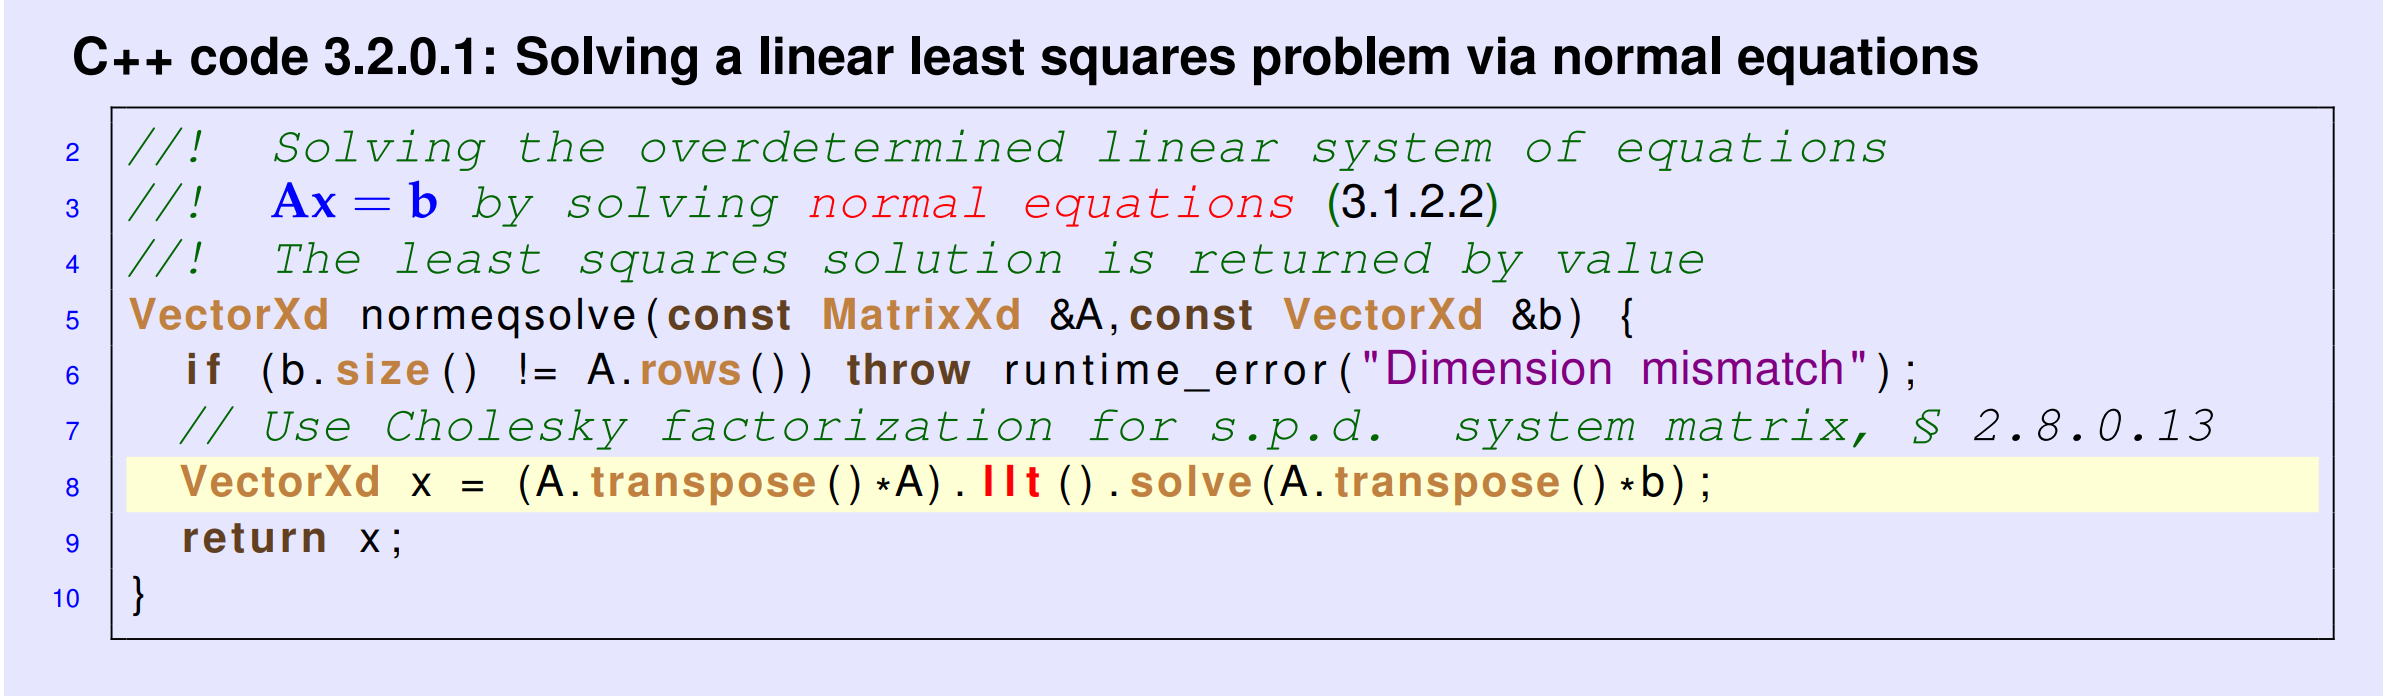
\includegraphics[width=1.0\linewidth]{NormalEquationsLinearLeastSquares.png}
\end{figure}
\noindent This produces the following helper function and the function itself.

\begin{figure}[!hbt]
    \centering
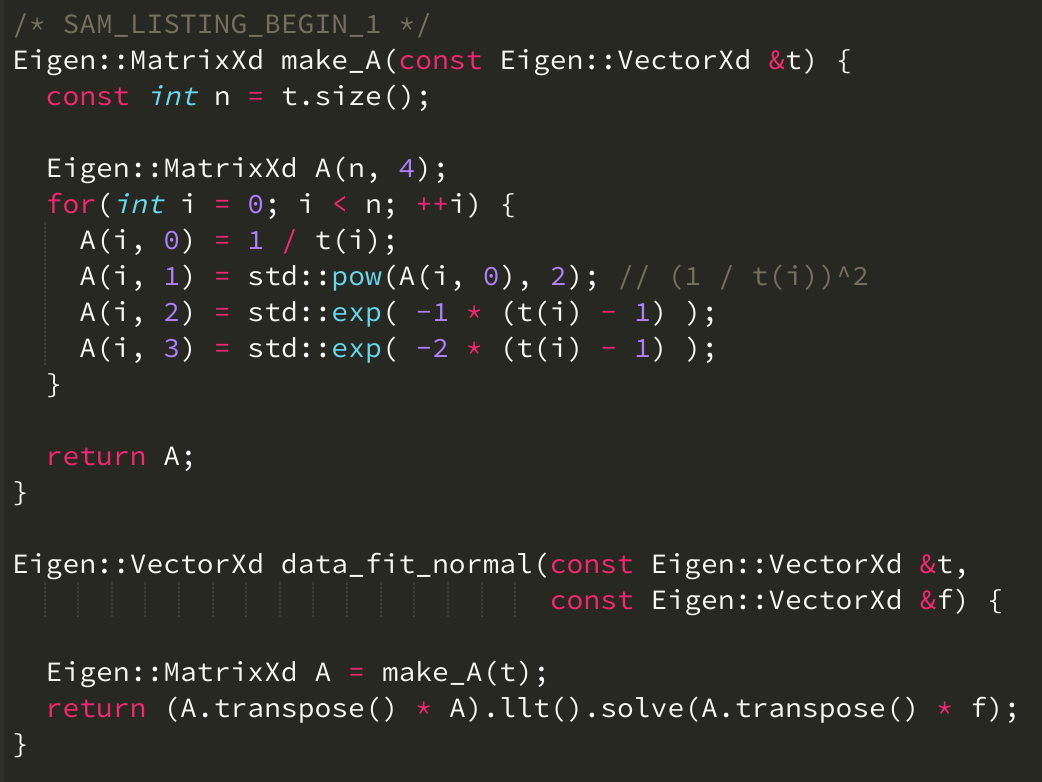
\includegraphics[width=1.0\linewidth]{3-3.a.png}
\end{figure}

\subsection*{3-3.b}
We are now tasked to use the orthogonal transformation techniques discussed with QR-decomposition for the same task as in 3-3.a. We can use the the \verb|HouseholderQR| functionality of Eigen here.

\pagebreak

\noindent We will again use the lecture document as guide, this time we use the code segement under 2.5.0.8 in the script (page 155). We can use the direct QR decomposition via function call on a matrix given to us by \verb|colPivHouseholderQR()| here as well, but this works as well.
\begin{figure}[!hbt]
    \centering
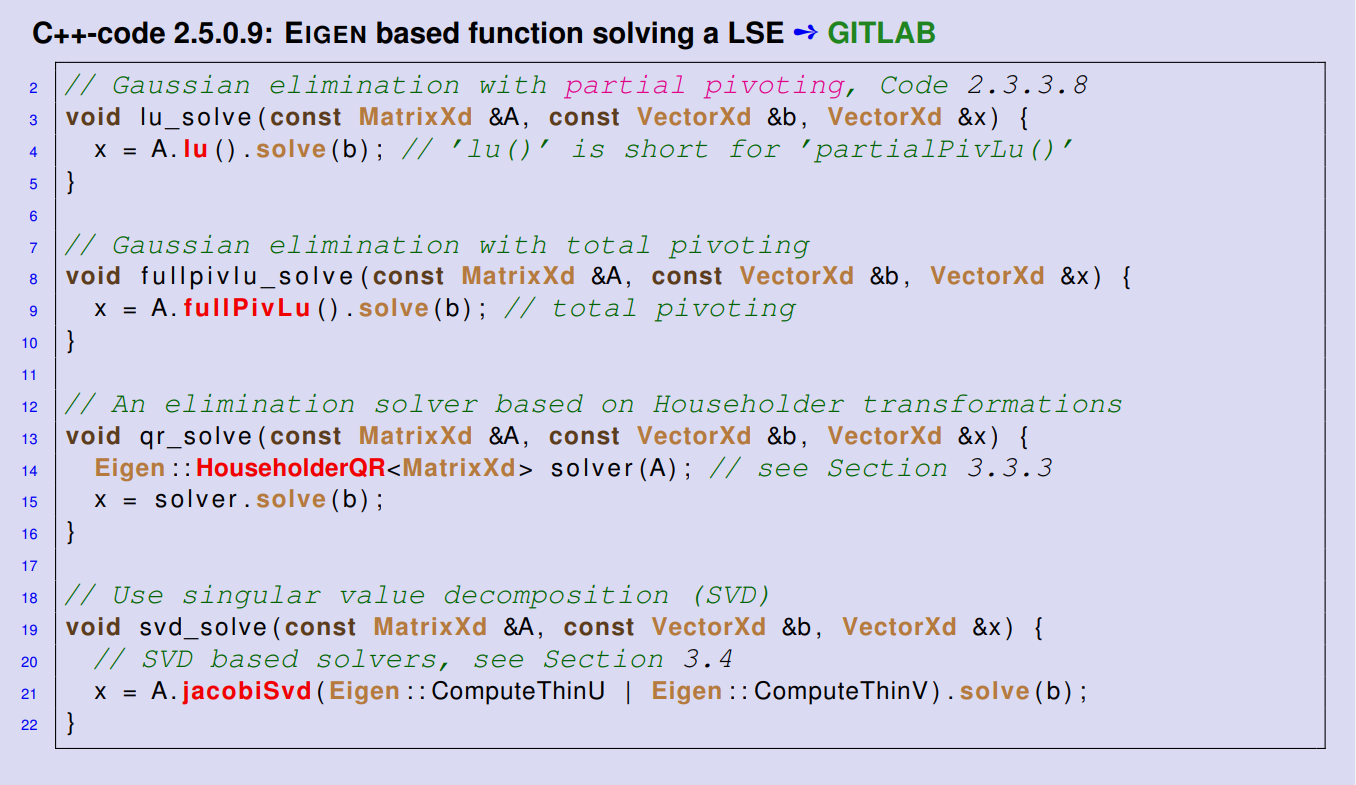
\includegraphics[width=1.0\linewidth]{SolversInEigen.png}
\end{figure}

\noindent This gives us the following code
\begin{figure}[!hbt]
    \centering
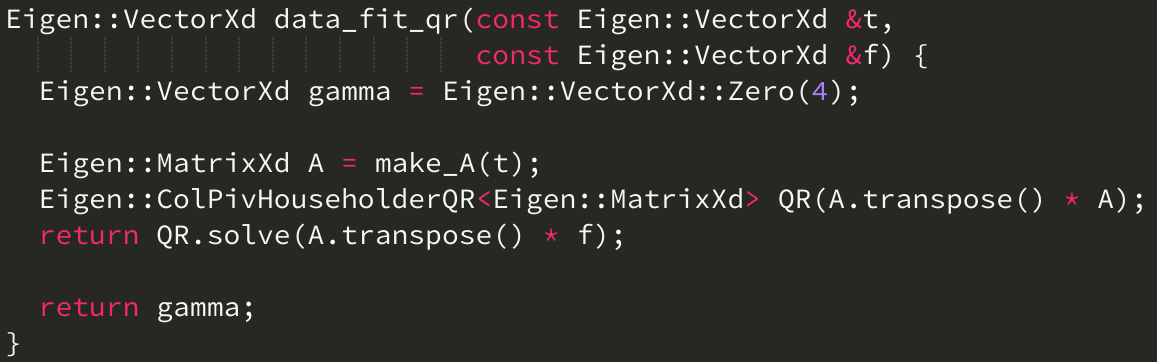
\includegraphics[width=1.0\linewidth]{3-3.b.png}
\end{figure}

\subsection*{3-3.c}
We are tasked with implementing a function that computes the function $f$ according to
\begin{equation*}
    f\left(t\right) = \sum_{j=1}^{4}\gamma_{i}\phi_{j}\left(t\right)
\end{equation*}
We will use this opportunity to directly practice our functor implementation skills. In an exam one would just compute \verb|make_A(t_vec) * gamma| (please use this), as this is the equation we derived from evaluating the function at the points. 

\pagebreak

\noindent This produces the following code, which was used to repeat the usage of functors and one should rather use the approach above.

\begin{figure}[!hbt]
    \centering
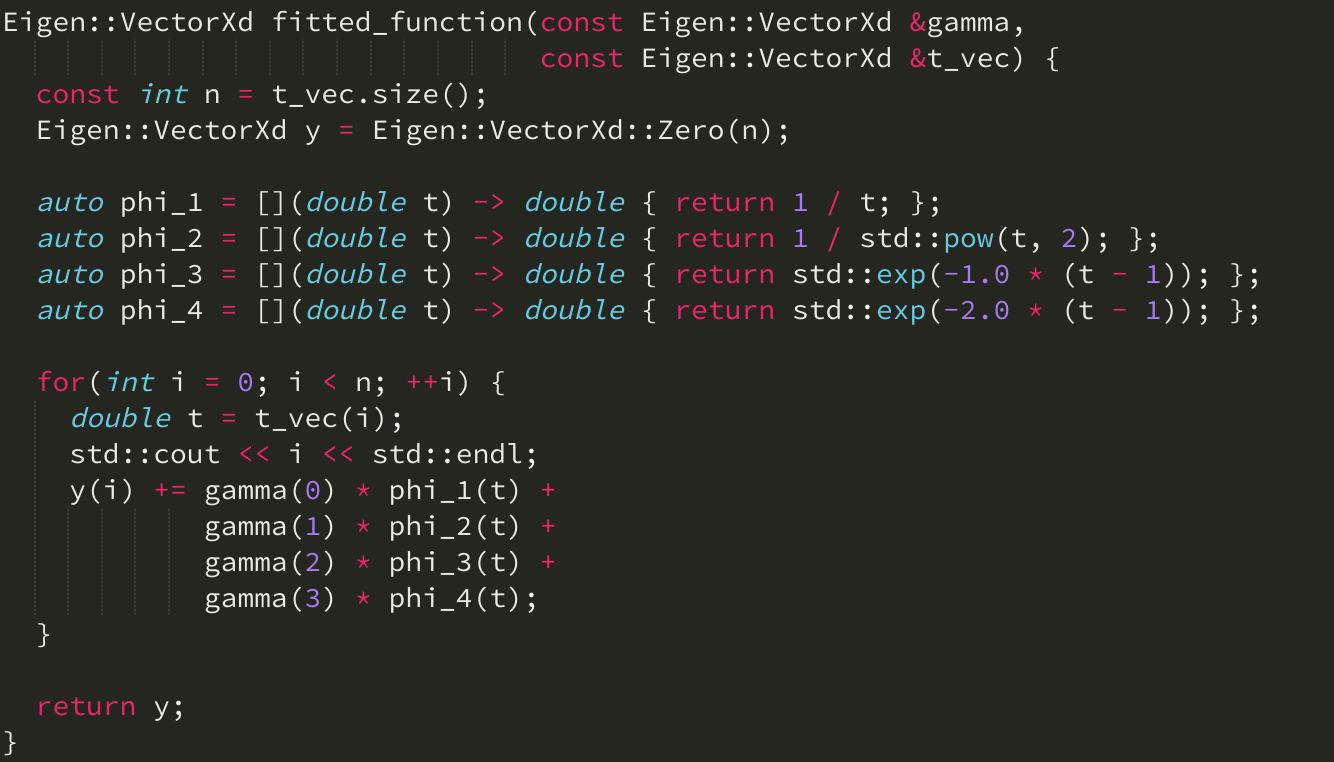
\includegraphics[width=1.0\linewidth]{3-3.c.png}
\end{figure}

\subsection*{3-3.d}
We are now tasked with implementing a function \verb|fitting_error| that returns the vector
\begin{equation*}
    \left[\left(f\left(t_{i}\right) - f_{i}\right)^{2}\right]_{i=1}^{10} \in \mathbb{R}^{10}
\end{equation*}

We use the following values given in the task description.

\begin{figure}[!hbt]
    \centering

\includegraphics[width=1.0\linewidth]{3-3Values.png}
\end{figure}

\noindent We now also use that $f\left(t\right)$ gives us the measured data points and $f_{i}$ gives us the points the fitted function computes, hence we use the \verb|fitted_function| with parameters \verb|gamma| and \verb|t_vec|, to do exactly this.

\pagebreak

\noindent Since we compute the squares of the difference for all then values, and the values represented in vectors, we take the difference of the two vectors and then use \verb|cwiseProduct| with the vector itself do directly compute all results without needing any for-loop. This gives us the following code.
\begin{figure}[!hbt]
    \centering
\includegraphics[width=1.0\linewidth]{3-3d.png}
\end{figure}

\noindent Here \verb|100.| is the shorthand notation for \verb|100.0|.


\end{document}
